% Do not change the options here
\documentclass[bsc,frontabs,singlespacing,parskip,deptreport]{infthesis}
\usepackage[utf8]{inputenc}
\usepackage{enumerate}
\usepackage{tikz}
\usetikzlibrary{arrows,shapes.gates.logic.US,shapes.gates.logic.IEC,calc}
\usepackage{hyperref}
\usepackage{aurical}
\usepackage[T1]{fontenc}
\usepackage{color}
\usepackage{enumitem}
\usepackage{listings}
\usepackage{wrapfig}
\usepackage{caption}
\usepackage{setspace}
\usepackage{geometry}
\usepackage{natbib}
\usepackage[toc,page]{appendix}
\setcitestyle{square} 
\geometry{a4paper,  margin=1in}
\definecolor{dkgreen}{rgb}{0,0.6,0}
\definecolor{gray}{rgb}{0.5,0.5,0.5}
\definecolor{mauve}{rgb}{0.58,0,0.82}
\begin{document}
\begin{preliminary}

\title{Stablecoins with an Analysis of MakerDAO and Dai}

\author{Samir Farhat Dominguez}

\course{Electronics and Computer Science}

\project{4th Year Project Report}

\date{\today}

\maketitle

\chapter*{Abstract}
With the rise in adoption and coverage of cryptocurrencies, a mainstream market still finds itself hesitant to participate, much preferring the storied, highly regulated and centralized currencies controlled by central banking systems. This is due in no small part to the quick and dramatic shifts in price for even some of the most widely adopted cryptocurrencies, most notably Bitcoin. As such, their have been numerous promising developments around blockchains and cryptocurrencies solely focused and designed on the ethos of stability. But what is stability? And how do we attain it? This work will seek to answer these questions
\smallbreak
\noindent
This report will begin by introducing the technical, historical and economical background surrounding cryptocurrencies. Subsequently, an explanation and enumeration of the subset of cryptocurrencies known as stablecoins will take place. Additionally, the Maker Foundation and its associated stablecoin 'Dai' will be described, in addition to the mechanisms and infrastructure which these entities are built on. The report will then follow with an elaboration of the implementation component, alongside a discussion of why this implementation is pertinent and imperative to the objectives of this year long investigation. These objectives being a critique of the Maker Foundation's work and an elaboration of the ideal definition of stability and the ways by which this definition is achieved. Finally, analysis of the implementation and its performance, which will serve to evaluate the performance of Dai's stability mechanisms, and how they perform against a more ideal notion of stability. 
\newpage

\section*{Acknowledgements}
Will write shortly before final submission...

\tableofcontents
\end{preliminary}


\chapter{Background and Introduction}
    \section{Cryptocurrencies}
    In order to contextualize this this work, it is first imperative to discuss the definition and history of cryptocurrencies. 
    \subsection{Definition and Motivation}
    A cryptocurrency is properly understood as a digital asset that works as a medium of exchange for goods, services, and other currencies. Records of ownership, transaction, and distribution of these currencies are stored in highly cryptographically secure databases known as blockchains. They have the marked characteristic of only existing in digital form, being decentralized, and are not to be confused with highly regulated, centralized, government-issued digital currencies, which are typically under the prerogative of central banking systems. 
    \smallbreak
    \noindent
    Blockchains are fundamental to the construction of cryptocurrencies, as they represent a distributed ledger which holds all records of movement and ownership of the cryptocurrency they pertain to. A blockchain, as the name entails, is a sequence of blocks linked cryptographically, usually by hashing the timestamp associated with each transaction. These blocks each contain information on each individual transaction or production of the cryptocurrency they maintain. They use separate computers which function as nodes that record, share and synchronize the transactions in their respective electronic ledgers. This is what allows cryptocurrencies to maintain their decentralized characteristic, as multiple devices across a network which verify and check against each other to ensure the blockchain has not been modified or tampered with by an outside entity. This characteristic, alongside strong cryptographic protocols, make blockchains almost completely resistant to modification, which is inimical to ensuring the security and reliability of the blockchain. Users and programs can interact with a blockchain through a construct called a smart contract.
    \smallbreak
    \noindent
    In the context of blockchains, smart contracts represent programs that delineate transaction protocols. Essentially, they are highly secure algorithms that control the distribution and ownership of a cryptocurrency. The network of nodes that maintain the blockchain verify that the smart contracts have not been tampered with. A simple example of a smart contract process would be when a fee payment is made to the Ethereum blockchain. When a user completes a payment, a program sends the record of this transaction to a smart contract, which updates the blockchain to include this movement of funds and issues the corresponding Ethereum to the cryptocurrency wallet associated with the user. This transaction record is then synchronized with all the nodes in the blockchain.
    \smallbreak
    \subsection{History and Rationale}
    \noindent Although cryptocurrencies are a contemporary construction they still have a more extensive history than a layman may be privy to. In the 1980s there was the so called 'first wave of crypto' where there was an attempt to digitize government issued currency. This venture was ultimately unsuccessful as the centralized nature of fiat currencies did not allow for a digital asset existing without a physical store of money to back it. However, these digital currencies would not fall under the definition of cryptocurrency delineated at the beginning of this subsection. This early period was valuable in defining some of the computational and engineering practices in the construction of modern cryptocurrencies. Some examples of this would be the creation of the first digital ledgers, the first coin mining operations, and the first successful transactions of completely digital assets(not backed by physical money in banks and reserves). 
    \smallbreak
    \noindent
    The 'second wave of crypto' led to the creation of cryptocurrency as we have defined it. The first and perhaps most significant of which was  Bitcoin. This led to the creation of separate currencies operated and distributed by independent parties, thus leading to the dozens of coins on the crypto-market we see today. This also led to the development of 'gimmick' coins, which are cryptocurrencies that are designed for advertising, single use, or only usable for specific merchandise distributors. Some examples of these include E-gold, used by 'cash for gold' businesses, or 'CryptoKicks' which is a purely promotional coin used to make purchases with the sportswear company Nike. The scope of this work will disregard these, as despite being registered as legitimate cryptocurrencies their functionality and usage makes them wholly irrelevant to this work's objectives.
    \smallbreak
    \noindent
    Right now, there is a pseudonymous 'third wave'. This exists in the form of stablecoins, driven by the need to stop mitigate the extreme volatility seen in most cryptocurrencies. This volatility is exemplified in Figure 1. This depicts Bitcoin dramatically shifting in comparison to that of centralized currencies, in this case the euro, British pound and Australian dollar. 
    \begin{figure}[h]
    \centering
      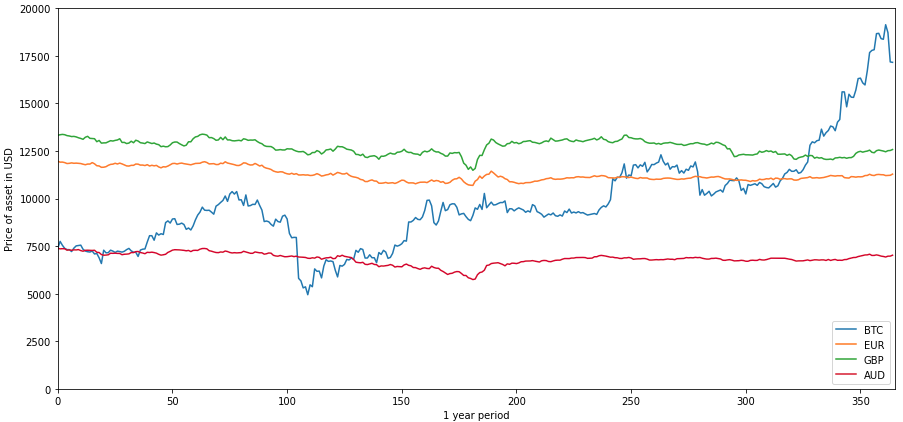
\includegraphics[width=\linewidth]{Images and Figures/bitcoinvsfiat.png}
      \caption{Bitcoin vs the USD and Fiat currencies vs 10,000 USD}
    \end{figure}
    \section{Stablecoins}
    Stablecoins are cryptocurrencies whose design and construction is primarily centered around the notion of maintaining a consistent value.
    \subsection{The Notion of Stability}
    Stability is often quantified in terms of its value relative to other fiat currencies. However, the concept of stability is a multifaceted and a somewhat vague concept. As such, their have been several different definitions of stability that can be targeted when designing a stablecoin. 
    \smallbreak
    \noindent
    The most common form of stablecoin proposals attempt to match the price of a single fiat currency. Most of the time the fiat currency selected is that of a global market hegemony. As such, stablecoins that match the price of the US dollar are the most common. Some examples of these are Tether, Dai, TrueUSD, BitUSD, and many others. The euro, British pound, and others also have stablecoin counterparts, although far and few between. Euro-STASIS and BinanceGBP are examples of these respectively.
    \smallbreak
    \noindent 
    Another conceptualization of stability that exists is that of stability with respect to a 'basket' of assets. These stablecoins select a subset of fiat currencies which are then weighted against each other to determine the value the coin should aim for. The most notable example of this type of stablecoin is that of Facebook's Libra. Libra is not currently live, but the proposal uses US treasury securities as well as the US dollar, euro, yen, British pound, and Singapore dollar in determining its target price. The weightings of these currencies on the target price is at the discretion of those who develop the coin. Weightings are often decided by examining the strengths, weaknesses, and volatility of the different currencies involved in calculations. As an example, the most recent proposal of Libra seems to weigh the USD as half of its price while the euro, yen, British pound and Singapore dollar compose the next  18, 14, 11, and 7 percent respectively. 
    \smallbreak \noindent
    Another form of stability is that of consistency relative to exchange-traded commodities. These exchange-traded commodities almost always take the form of precious metals such as gold and silver or natural exhaustible resources such as petroleum. Some cryptocurrencies tied to the price of drinking water have been proposed as well. These currencies can use a 'basket' model as well, where several assets are weighted to calculate a target price. These coins are more robust against crisis or inflation, since they are at the behest of tangible physical assets, rather then the more abstract prices traditional fiat currencies can take. That being said, physical assets can see changes in supply and demand, and thus run the risk of volatility in purchasing power. A strong example would be the almost inevitable depreciation of the price of petroleum, as more and more nations incentive the ownership of electric motor cars. 
    \smallbreak \noindent
    Finally there is stability with respect to inflation. This form of stability seeks to maintain constancy relative to market indicators rather than assets. The strongest example of these would be Anchor, a cryptocurrency that pegs itself to a value derived from the Monetary Measurement Unit, an economic notion derived from a series of macroeconomic inflation indicators. 
    \subsection{Supply and Demand}
    Now that we understand the different pegs and target prices that a stablecoin can seek to achieve, it is imperative to discuss the most fundamental underlying principle that allows for a target value to be achieved. This is the economic principle of supply and demand.
    This discussion will assume a single market and a linear relation between supply and demand. Most real life environments have complex factors that impact supply, demand, and prices. These factors escape the scope of this work. 
    \smallbreak \noindent
    Supply is the total amount of a good or service that is available to market consumers. The law of supply states that the higher the price of a good or service, the higher the supply of that good or service will result in a given period of time. In a linear environment this relation is described mathematically as follows: \[(p - p')(y - y')\geq 0\] Where \(y'\) is the supply of an asset at lower price \(p'\), and \(y\) is the supply of an asset at higher price \(p\).  
    \smallbreak \noindent
    Demand is the quantity of a good or service that consumers are willing to purchase at various prices during a given period of time. Therefore, the law of demand states that as the price of a good or service changes, the demand of that good or service will shift inversely. Ergo, higher prices decrease demand, and lower prices increase demand. In a linear context, this results in the following mathematical relationship: \[d(p) - d(p') > 0\] Where \(d\) is a function of the demand of a good or service, \(p\) denotes a higher price of a good or service, and \(p'\) is a lower price for the same good or service. Putting these two fundamental economic terms together, one can observe that both these factors have a relationship with the price of goods and services, and this mutual relationship can be modelled (in a linear environment) by the below supply and demand curve. 
    \begin{figure}[h]
    \centering
      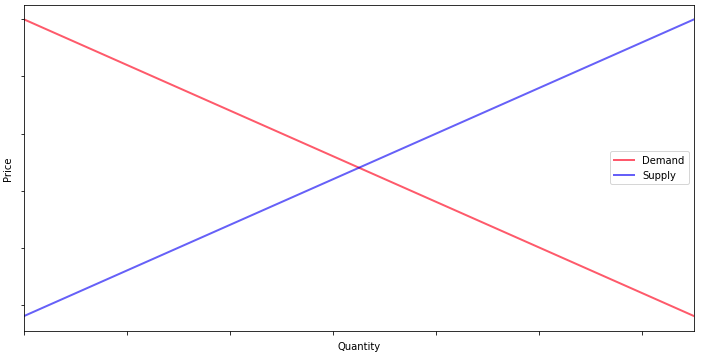
\includegraphics[width=\linewidth]{Images and Figures/supplyanddemand.png}
      \caption{Supply and Demand Curve}
    \end{figure}
    \smallbreak \noindent
    Taking this supply and demand curve, it is important to understand that the intersection of the demand and supply line is called the equilibrium point. This equilibrium is of paramount importance, as it represents the point at which the value and quantity of an asset stabilizes. Now, if one takes this phenomena and extrapolates it to a stablecoin, where the supply and demand can be controlled either directly through the blockchain, or indirectly through incentives, then one can seek to build mechanisms that lead to desired equilibrium points. As an example, let us say tether, a directly backed stablecoin pegged to the USD can now be purchased for 0.993 USD, meaning it is slightly below its target price of 1.000 USD. If the blockchain where to decrease the network commission of transactions(say from 0.2\% to 0.18\%). This would mean that the demand for Tether would increase, as it has become effectively cheaper to purchase. Naturally, the demand would increase such that the equilibrium point occurs at a higher price(ideally 1.000 USD). This sort of indirect or direct influence on supply and demand is the way by which all stability mechanisms seek to align their stablecoins with their target price. 
    \subsection{Stability Mechanisms}
    Having discussed the concept of stability, one can move forward by elaborating on the different methodologies employed to achieve a consistent coin value. There are two principal types of Stablecoins, backed and intervention-based.
    \smallbreak \noindent
    Backed stablecoins are characterized by having a reserve of money that functions as collateral to the value of the coin. That is to say a coin has assets that act act as a guarantee or security in case of a significant drop or total dissolution of the coins value. These coins come in two subsets, namely indirectly backed and directly backed. Indirectly backed coins use currencies not within their target asset or basket of assets as collateral. This can be a separate fiat currency or another cryptocurrency, commonly an Ethereum-based token. Directly backed stablecoins maintain a reserve of the target currency, often in excess of the market cap of the coin. This means that if a stablecoin pegged to say the US dollar has a market cap of 1 billion USD, then the reserves will often hold 1.3 to 2 times that value in order to ensure the robustness of their coins value. Directly backed coins can also be redeemable by the public or only the centralized entity that created the coin, which means it is important to distinguish directly backed and directly backed redeemable coins, as the former does not hold the benefit of public usability while the former does. This calls into question the legitimacy of directly backed coins being considered legitimate cryptocurrencies, but that discussion escapes the scope of this work.
    \smallbreak
    \noindent 
    Intervention-based stablecoins maintain stability through algorithmic and human intervention mechanisms. A trusted oracle will track the price of the coin and then make adjustments to ensure the constancy of the coins price relative to the asset it targets. A simple example of this would be in the blockchains releasing of the coin. If a large amount of the currency is released but the demand for the coin does not increase, then the law of supply and demand will lead to the depreciation of the coins value. At this point, the oracle might then repurchase or freeze transactions to create a scarcity, which will in turn lead to an increased price as the supply drops to meet the demand. In the following table there is a quick summary of how these stablecoins compare to other currencies in terms of decentralization and stability.
    \begin{table}[h]
    \centering
      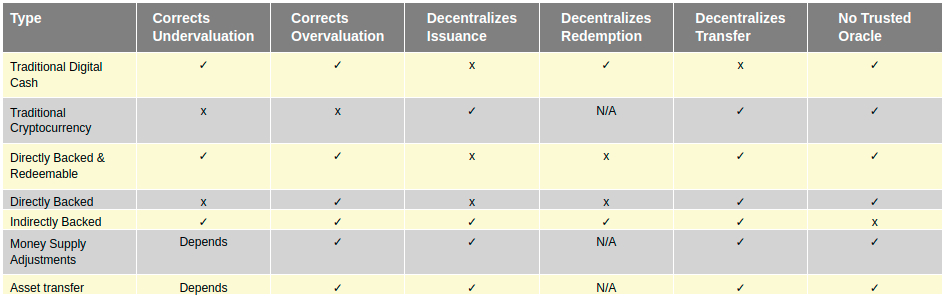
\includegraphics[width=\linewidth]{Images and Figures/coinmech.png}
      \caption{Digital currencies and their characteristics}
    \end{table}
    \smallbreak \noindent
    \smallbreak \noindent 
    There are a myriad of mechanisms and combinations of approaches. These will be listed, followed by a brief enumeration and description of the largest stablecoins on the market. 
    \begin{itemize}
        \item Correcting undervaluation: Undervaluation corrected can be done in an innumerable amount of ways. However, this is principally executed by limiting the supply of the stablecoin. Naturally, this is based on the economic principal of supply and demand. 
        \item Correcting overvaluation: Increasing supply leads to the asset being valued at less. Once again based on the principal of supply and demand.
        \item Decentralizing issuance, redemption, and transfer: Spreading control of an asset amongst a large amount of people in a free market allows for a currency to stabilize. This is highly complex, but since the goal of a stablecoin is to be widely adopted, it is worth the complexity. 
        \item Trusted oracles: Oracles are networks that set parameters for the blockchain a stablecoin is based on. These can be highly sophisticated and complex modules, or be as simple as a line of code that tracks a number.
        \item Arbitrage: Arbiters essentially mimic high rollers in a blockchain. They hold a high proportion of the asset, and are therefore able to control the price of a stablecoin by hoarding or dumping. This is similar to the mechanism of controlling under and overvaluation, but is more ethically suspect. 
    \end{itemize}
    \begin{table}[h]
      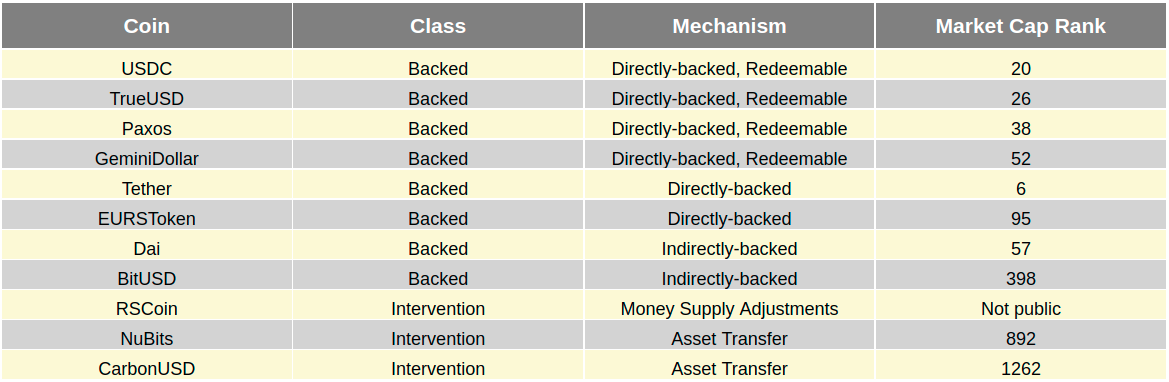
\includegraphics[width=\linewidth]{Images and Figures/coinproposals.png}
      \caption{Stablecoin proposals and their classification}
    \end{table}
    These mechanisms allow stablecoins to maintain a consistent value relative to the asset they choose to peg themselves to. This is exemplified in the figure below, where the most widely adopted stablecoin Tether(USDT) maintains an almost perfectly consistent value of 1 USD.   
    \begin{figure}[h]
            \centering
         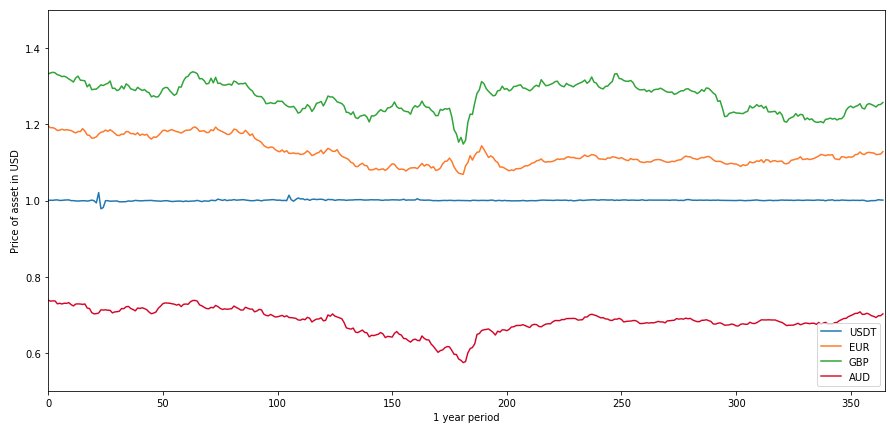
\includegraphics[width=\linewidth]{Images and Figures/tether.png}
              \caption{Depiction of the value of Tether in comparison to Fiat currency}
              \label{fig:boat1}
    \end{figure}
    \section{MakerDAO, Maker Protocol and Dai}
     The bedrock this work will build on is the MakerDAO foundation and their development of the stablecoin 'Dai'. Therefore, it would be pertinent to elaborate on the systems and goals of MakerDAO, as these will be critiqued later on in the work.
    \smallbreak
    \noindent The creation of MakerDAO and Dai was principally motivated by a distrust of biased and dysfunctional centralized financial system. As a result, it has the end goal of decentralization, transparency and is managed by users all over the world. Its blockchain is built on top of a network of servers that require collective verification, meaning the blockchain cannot be altered unless every computer in the network agrees on a change. This makes it highly secure and resistant to malicious actors. Relative to other stablecoin proposals it has been immensely successful. It currently has one of the largest market shares of any nominal stablecoin, and has a highly active and committed user base.
     \smallbreak
     \noindent The Maker foundation has permitted Dai to be used as a standard currency. Allowing for the storing of money in the blockchain, which is a vital function for any cryptocurrency to attract investment. It can also be used as a medium for exchange, a standard of deferred payment in the Maker protocol, and a unit of account in the Maker protocol.  The Maker protocol allows users to generate Dai, a stablecoin that has a soft peg to the US dollar. Specifically, it seeks to be valued at exactly 1 USD. This means that Dai defines its stability around a single fiat currency.
    \smallbreak
    \begin{figure}[h]
            \centering
         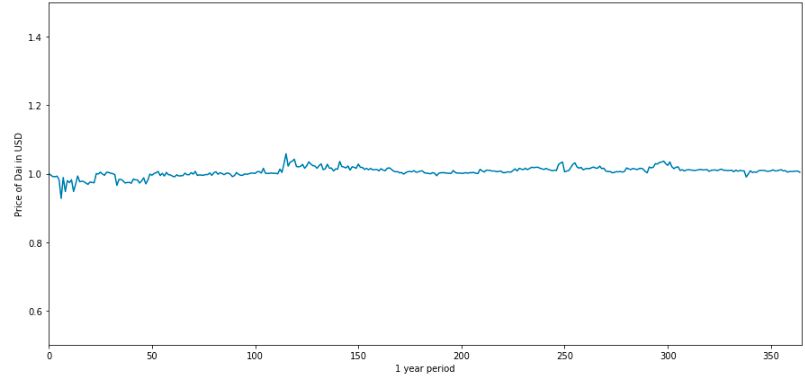
\includegraphics[width=\linewidth]{Images and Figures/dai.png}
              \caption{Value of Dai over the last year}
    \end{figure}
    \smallbreak
    \noindent
    The Maker Protocol is a multi-faceted system, held together through a collection of different stakeholders with varying interests, incentives, and responsibilities. The figure below presents a use-case diagram of the maker protocol. This presents the stakeholders involved in the maker protocol and their enumerated interests and roles within the maker foundation. These entities, their interests, and responsibilities will be explained thoroughly in the next few subsections. However, taking some time to parse through the diagram below will be very helpful in contextualizing the at first intimidating phraseology and components of the maker protocol. 
    \smallbreak
    \begin{figure}[h]
            \centering
         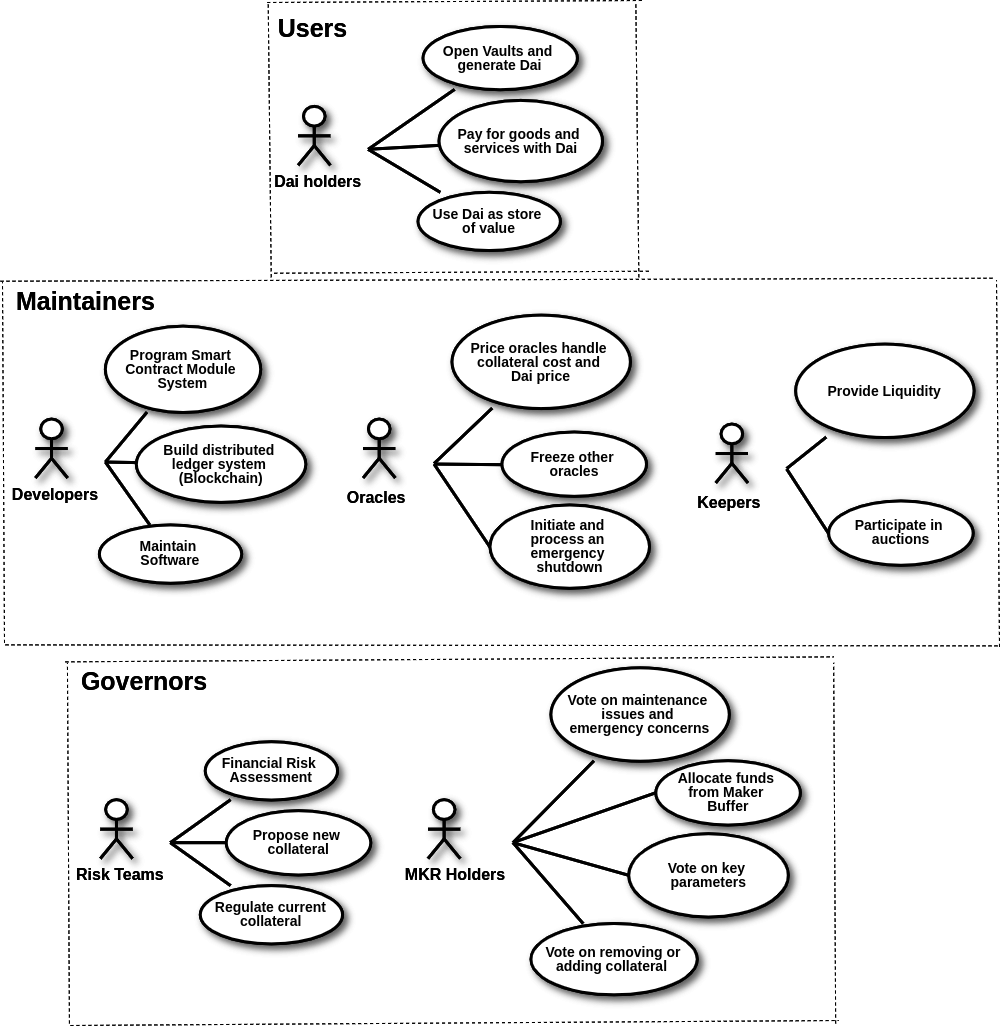
\includegraphics[width=\linewidth]{Images and Figures/Use Case Diagram.png}
              \caption{Maker Protocol use-case diagram}
    \end{figure}
    \smallbreak \noindent
    To begin detailing the different systems and players involved in the maker protocol, it would be reasonable to begin by explaining how Dai is 'minted'. This takes place through the end user's interaction with Maker vaults.  
    \subsection{Maker Vaults}
    \smallbreak \noindent
    For the creation of Dai to take place, a user creates and deposits Ethereum-based currencies in Maker vaults. These vaults are non-custodial, meaning that only the creator has control over the stored assets unless a liquidation occurs.  The life cycle of a vault is described in the list below.
    \begin{itemize}
        \item A user opens a vault through a community created interface or API.   
        \item The user specifies the amount of Dai they wish to withdraw, and then deposits an Ethereum-based currency into the vault. The allowed Ethereum-based currencies and the amounts are determined by Maker governance and oracles respectively (more on these entities later). Once the user deposits the currency the vault is considered collateralized. This means the system has a reserve that backs the created Dai. 
        \item While the vault a set of parameters will constantly update in accordance with governance and oracle regulations. The first of these is the stability fee, which generates interest on the Dai that has been withdrawn until the user closes the vault. The user closes the vault by giving back the Dai, retrieving their collateral, and paying the stability fee. 
        \item The second and most important parameter is the collateral to debt ratio, defined as a ratio between the price of the collateral and the withdrawn Dai. Once this ratio becomes too small, as determined by the liquidation ratio set by Maker governance, the collateral is deemed to not be enough to collateralize the missing Dai, and the vault is liquidated.
        \item A Maker vault liquidation takes place by an internal Maker Protocol Auction, where Dai holders are allowed to bid their Dai for the collateral that the vault holds. The auction must generate enough Dai to cover the vault's outstanding obligations, meaning the original generated Dai and the stability fee. The auction can either result in the vault obligations not being covered, vault obligations being covered with the auction of all the collateral, or vault obligations being covered with some of the collateral 
        \item If the vault obligations are not covered in the deficit is converted into Protocol debt, which is covered by Dai in the Maker Buffer, a reserve of Dai held by the Maker governance with the purpose of handling deficits. the amount of Dai in the Maker Buffer is determined by the Maker governance, and ideally holds enough funds to cover deficits incurred. Finally the user pays a liquidation fee before the vault is closed
        \item If more than enough is made in the auction to cover obligations of the vault, the remainder after the liquidation fee goes to the vault owner before the vault is closed. 
        \item If just enough is made in the auction to cover the vault's obligations, the user pays a liquidation fee before the vault is closed. 
    \end{itemize}
    \smallbreak \noindent
    It is important to know that throughout the steps above any movement of Dai is recorded and verified in the blockchain. The life cycle of a typical vault is depicted in the sequence diagram below
    \begin{figure}[h]
            \centering
         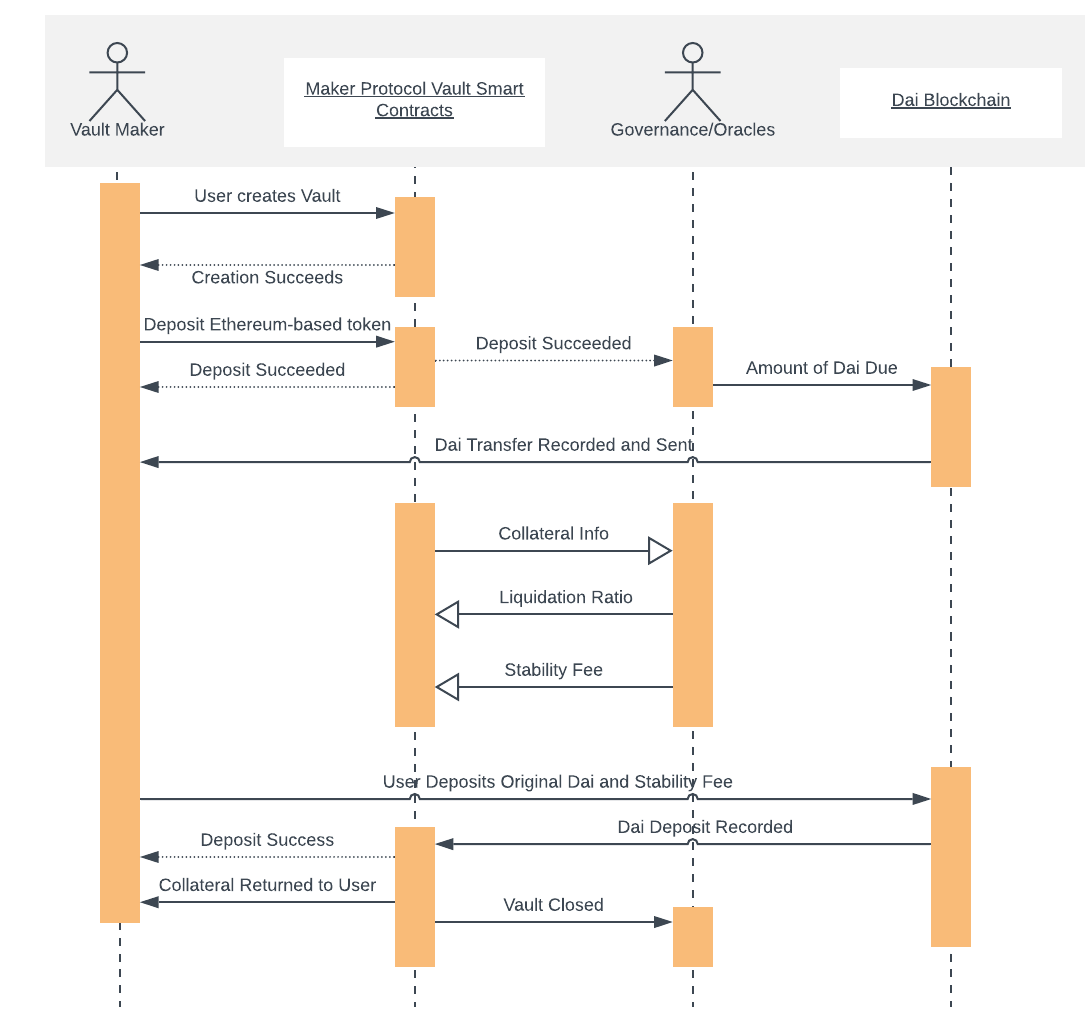
\includegraphics[width=\linewidth]{Images and Figures/Sequence Diagram Typical Vault.png}
              \caption{Sequence Diagram of a Typical Vault's Life cycle (No liquidation or auction)}
    \end{figure}
    \subsection{Governance}
    \subsubsection{MKR Holders}
    One of the ways  the Maker Foundation has managed to maintain decentralization is by delegating governance with the Maker token (MKR). MKR is a separate cryptocurrency, and can be thought of as shares of influence in the Maker protocol. MKR holders can submit proposals for voting and participate in polling for proposed changes to the protocol. MKR also serves as a recapitalization asset as the blockchain increases its supply if debt accrued on Dai exceeds the surplus MKR used to cover that debt. The price of MKR is therefore intrinsically tied to the health of the Maker protocol and the stability of Dai, functioning as an incentive for MKR holders to govern responsibly. See the diagram below for a depiction of the MKR token's value in the last year. 
    \begin{figure}[h]
            \centering
         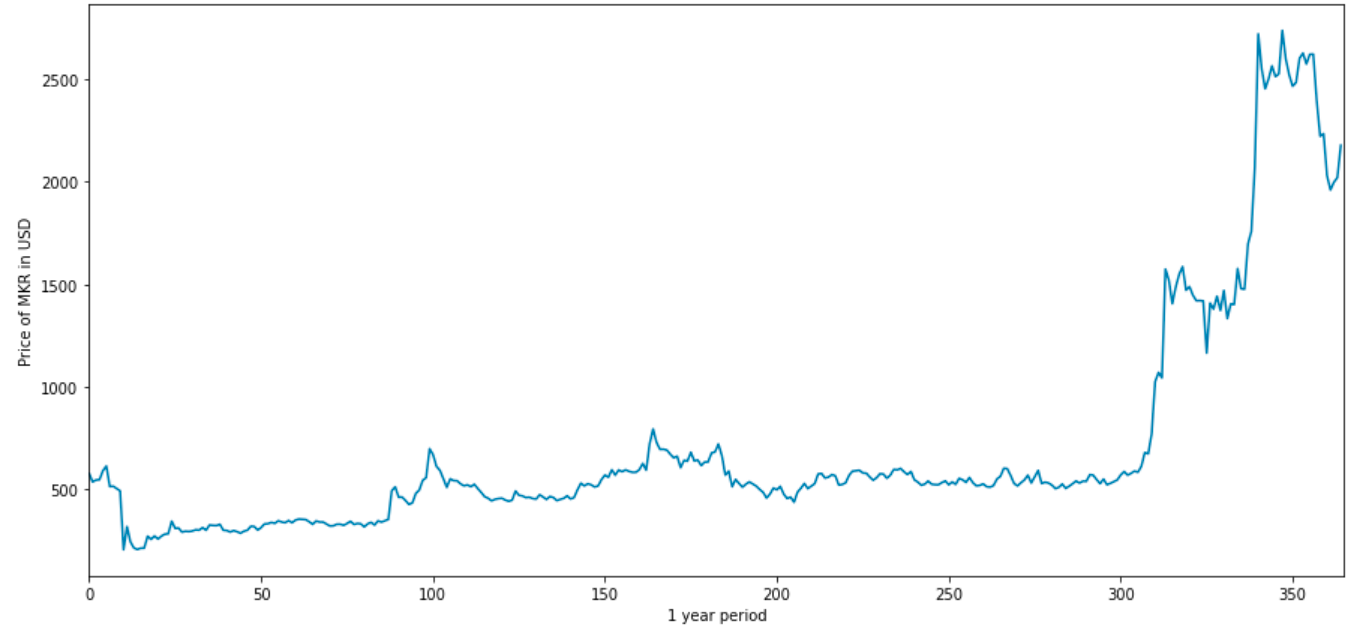
\includegraphics[width=\linewidth]{Images and Figures/mkrprice.png}
              \caption{Price of Maker Governance Token over the last year}
    \end{figure}
    \smallbreak \noindent 
    MKR holders can choose emergency oracles, trigger emergency shutdowns, allocate funds, upgrade the system, activate the governance security modules in case of an attack, and other important responsibilities. Amongst these responsibilities, MKR holders also vote on the parameters relating to debt ceilings, stability fees, liquidation ratio of vault assets, liquidation penalties, collateral auction duration, auction step sizes, and the Dai savings rate for those making interest on their Dai. 
    \subsubsection{Risk Teams}
    Risk teams are incentivized by payment from the Maker foundation. They perform comprehensive analyses and producing reports for MKR holders. These reports help MKR holders make informed decisions about what collateral types vaults should be allowed for vault making and regulations on the risk margins associated with different collateral relative to Dai. 
    \subsection{Maintainers and Oracles}
    The Maker protocol also relies on key external actors as well as automated systems called oracles, regulated by governance as well as maintainers.
    \subsubsection{Oracles}
    The Maker Protocol has a decentralized oracle infrastructure. This infrastructure consists of a set of nodes called oracle feeds. These oracles are protected by the oracle security module, which functions as a verifier to ensure that oracles have not been tampered with by non-approved actors. 
    \smallbreak \noindent
    The oracles that exist in these oracle feeds are selected by Maker governance, and have varying roles in maintaining the stability of Dai and the Maker protocol as a whole. A large proportion of these oracles deliver relevant information to Dai users and Maker governance, this information can include the total supply of Dai, the frequency and size of Dai transactions, the parameters of different types of vault collateral, etc. 
    \smallbreak \noindent 
    Some of the most important oracles in the system are the emergency oracles, which can freeze problematic oracles as well as trigger emergency shutdowns. Emergency shutdowns are a last resort stability mechanism that protects against attacks. It works by freezing price feeds, returning assets to vault owners and triggering massive post shutdown auction processes that take place to handle excess collateral. 
    \subsubsection{Keepers}
    Keepers are independent actors incentivized by arbitrage opportunities. They help maintain target price by dumping when above target price, and purchasing large supplies of Dai when below target price. They participate in surplus auctions, debt auctions and collateral auctions. Their principal incentive is the earnings they make through the Dai savings rate, which is a parameter determined by governance. Since keepers hold massive quantities of Dai, the interest accrued through Dai ends up earning these stakeholders a considerable return. 
    \subsection{Maker Protocol Future} 
    Understanding, the specific goals of the Maker Foundation and their namesake's protocol is not wholly relevant, all that one could say is that by evaluating the system and its underlying mechanisms one can critique the extent to which the Maker Foundation will be able to realize their ambitions. The Maker protocol has also outlined the following list of its objectives for the future of Dai.
    \begin{itemize}
        \item The protocol wishes to reach complete decentralization by outgrowing and gradually removing the need for the Maker Foundation and its operations. 
        \item It wishes to extend its addressable market by turning Dai into a standard savings and exchange currency used in the technology industry. Furthermore, this would turn Dai into a capital and hedging currency.
        \item Another ambition is to extend its market to charities and NGOs, as the transparent and unbiased nature of the Dai blockchain can help ensure accountability and non-profit status.
        \item The protocol also wishes to develop more sophisticated oracles that will be able to help MKR holders fulfill the responsibilities of the Maker Foundation.
    \end{itemize}
    
    \section{Objectives}
    \subsection{Objectives}
    \smallbreak \noindent 
    This work, its motivation, and its objectives can be summarised with the following two themes. Firstly, the text seeks to define the most sturdy definition of stability in the context of cryptocurrencies as stability relative to inflation, that being a cryptocurrency that can maintain its purchasing power consistent with market trends. Secondly, this work seeks to examine the mechanisms and infrastructure required to bring about said definition of stability. Since the Maker protocol has one of the most thoroughly developed stability mechanisms and infrastructure, it will serve as a cornerstone by which the implementation and analysis takes place. 
    \subsection{Stability and the Consumer Price Index}
    In selecting a peg that best represents inflation and purchasing power trends, the basket of goods, alternatively called the Consumer Price Index (CPI) is a natural choice. This index is a representation of the average household expenses in a given nation, region, or community. Most countries with the infrastructure to do so collect and publish data on the CPI in their specific nations, as this data has been proven to be the most reliable metric by which inflation is measured. As an example, the UK's central clearing bank, the Bank of England, uses the CPI to establish inflation goals, set monetary policy and determine the quantities of money to print. 
    \smallbreak \noindent
    The different products that constitute the CPI are determined on a yearly basis, and naturally change with market trends. As an example, the CPI has consistently included expenses like coffee, petrol, and electricity. However, over the last few decades, modern products relating to personal computers and the internet have been added, while outdated products relating to radio equipment and VCRs have been removed. Nonetheless, more inconspicuous products can be added and removed for much less intuitive reasons. For instance, in the CPI report of 2020 'Fruit Pies' were removed because "Its removal enables crumpets to be added, thus widening the variety of representative products in this part of the basket". 
    \smallbreak \noindent
    The ONS publishes detailed datasets relating to the CPI on a monthly basis. These datasets contain information as general as the CPI for a given month, down to the individual products and their weightings in CPI calculations. It includes yearly data since 1998, and monthly data since 2008.
\chapter{Implementation}
    \section{Proposal}
    The objective for the implementation component of this work will be the development of stability mechanisms for a new stablecoin, with the objective of achieving stability relative to inflation and purchasing power. The development of these mechanisms will employ a large number of the methods utilized by MakerDAO, and as such, serve as a critique of the MakerDAO foundation and its proposal's strengths and weaknesses. This Stablecoin will be dubbed Basket (BSKT) and will be an indirectly backed stablecoin targeting the price of the United Kingdom's consumer price index according to the Office for National Statistics (ONS). 
    \section{The Plan}
    As far as the scope of the implementation of the report, it would not be practical to strive to construct a fully functional public stablecoin from scratch. Putting aside the experimental nature of BSKT, just developing a fully secure and functional cryptocurrency could take a team of developers multiple years, as well as a monetary investment in the realm of tens of thousands of pounds. Since the objectives of this report relate to stability and the mechanisms by which this stability is achieved, the following implementation is proposed. The open source and public statistics, modules, and systems available from the Maker Foundation will be used to create a simulation environment whereby simulated stakeholders interact with these modules in the context of the CPI data available over different amounts of simulated time. Several considerations and parameter distributions will be evaluated in order to ensure a simulation environment that may best mimic reality. These will be developed subsequent to this section.
    \subsection{Maker Protocol without Dai}
    Germane to the Maker Foundation's dedication to transparency and decentralization, the full source code and architecture documentation that constitutes the Maker Protocol and Dai stablecoin smart contracts are public. This gives this work a considerable foundation with which to build the Basket mechanisms with modified versions of the Maker Foundation's mechanisms and systems. 
    \subsubsection{Additions}
    \subsubsection{Removals}
    \subsubsection{Modifications}
    \subsection{Target Price}
    \subsubsection{Consumer Price Index Data}
    \subsubsection{Incentives and the Application of Supply and Demand}
    \subsubsection{Accounting for Coronavirus and Brexit}
    One of the most important factors in creating a successful testing and analysis environments is to establish conditions that are normative and consistent. As such, the data and quantitative methods that will be used during the experimentation will ignore the 2021 ONS data, as the combination of the Brexit transition and Covid-19 outbreak have created a set of unique and unusual market conditions. While a public version of Basket should be robust enough to maintain its value in these specialized conditions, the temporal limitations and scope of this work are such that it would not be productive to engage with these outliers. The version of Basket that this work will seek to produce would be more accurately described as a minimum viable product (MVP), rather than any sort of public or consumer ready cryptocurrency.  
    \subsection{Simulation}
    \subsubsection{Data sets}
    \subsubsection{Defining Simulation Parameters}
    \subsubsection{Test Reporting}



\chapter{Analysis}
\section{Analyzing Results}
\section{Conclusion}
\section{Evaluation}
    \subsection{Limitations and Shortcomings}
    \subsection{Extensions and Future Work}
\bibliographystyle{plain}
\bibliography{Bib/bibliography}

\appendix
\chapter{CPI and ONS Data}

\chapter{Basket Code Snippets}

\chapter{Test Scripts, Parameters, and Data}

\end{document}